\documentclass[11pt]{article}
\usepackage[a4paper,margin=24mm]{geometry}
\usepackage[T1]{fontenc}
\usepackage{lmodern,microtype,amsmath,amssymb,amsthm,mathtools}
\usepackage{booktabs,array,graphicx,xcolor,enumitem,fancyhdr}
\usepackage[colorlinks=true,linkcolor=teal!65!black,citecolor=teal!65!black,urlcolor=teal!65!black]{hyperref}
\definecolor{ink}{HTML}{153044}\definecolor{accent}{HTML}{087F8C}
\setlength{\parindent}{0pt}\setlength{\parskip}{5pt}\setlength{\headheight}{15pt}
\pagestyle{fancy}\fancyhf{}
\fancyhead[L]{\small Quantum mechanics and general relativity: extensions}
\fancyhead[R]{\small Logan Voss}\fancyfoot[C]{\thepage}
\newtheorem{theorem}{Theorem}[section]\newtheorem{proposition}[theorem]{Proposition}
\newtheorem{corollary}[theorem]{Corollary}
\newcommand{\Tr}{\operatorname{Tr}}\newcommand{\dd}{\mathrm d}
\newcommand{\sech}{\operatorname{sech}}\newcommand{\arcosh}{\operatorname{arcosh}}
\newcommand{\arsinh}{\operatorname{arsinh}}\newcommand{\R}{\mathbb R}
\hypersetup{pdftitle={On Quantum Mechanics and General Relativity: Dynamical Extensions},pdfauthor={Logan Voss},pdfsubject={Selected reciprocal coupling, one-Killing selection, and sourced quadratic-curvature discrimination}}
\begin{document}
\hypersetup{pageanchor=false}
\begin{titlepage}
\vspace*{10mm}
{\color{accent}\small\scshape Research edition 2.0}\par\vspace{9mm}
{\color{ink}\Huge\bfseries On Quantum Mechanics\par and General Relativity}\par\vspace{8mm}
{\Large Logan Voss}\par\vspace{8mm}
{\large Dynamical coupling, one-Killing selection,\par and sourced curvature discrimination}\par\vspace{10mm}
\hrule\vspace{6mm}
\textbf{A compact relation.} For the selected centered quadratic probe and pure Gaussian preparation,
\[
\boxed{\Delta E=\hbar\omega(\mathcal F^{-2}-1),\qquad
\mathcal F=|\langle\psi_M|\psi_N\rangle|^2.}
\]
Its reciprocal shape source satisfies
\[
\boxed{\|\mathcal S\|_G^2=\Delta E(\Delta E+\hbar\omega).}
\]
The interaction is selected before solving a trajectory. A positive joint quantum model gives reciprocal response; a flat helical calibration selects a one-Killing gravitational action; and two sourced calibrations distinguish the constant quadratic-curvature alternatives.
\par\vspace{4mm}
All results have explicit model contracts. The complete formal package contains 63 theorems across nine modules and compiles with zero warnings and zero errors. Written proofs, symbolic identities, independent checks, and finite quantum simulations have distinct stated scopes.
\vfill
{\small November 13, 2026\par
Research with AI-assisted derivation, verification, formalization, and editing. All extension calculations and the bounded independent review were frozen before public authoring. No experimental observation or worldwide-priority claim is made.}\par
\end{titlepage}
\hypersetup{pageanchor=true}

\begin{abstract}
We extend a conditional quantum-state/geometry selection framework in three directions. First, calibrated common-frame covariance selects a target-only positive centered quadratic probe Hamiltonian. It fixes an exact energy--fidelity relation and a reciprocal shape source, including a covariance-uncertainty bound. Quantizing the shape cell gives a positive linear quantum model with symmetry-related preparations of identical joint-energy spectral measure and opposite initial responses of a bounded observable. Its instantaneous ground band has a computable Berry connection, Born--Huang correction, and exact initial leakage coefficient. Second, a flat helical reference selects the Einstein--wave-map action on a three-dimensional quotient with only one required Killing symmetry. A smooth-current variational extension exposes and repairs the sourced twist-reconstruction obstruction, fixing both mixed and contact terms. Third, within unrestricted four-dimensional constant-coefficient parity-even quadratic gravity with fixed sources, dust cosmology and charged electrovac calibrations select the Einstein bulk coefficients modulo the Euler density. Sourced response channels provide exact parameter inverses and model-consistency tests. These are conditional extensions with reproducible proofs and controls. The fully quantum cell model, covariant state-fluid model, and four-dimensional matter interpretation remain distinguished; no interacting constrained quantum-gravity continuum is asserted.
\end{abstract}
\setcounter{tocdepth}{1}\tableofcontents
\newpage

\section{What is extended, and under which assumptions}
The foundation~\cite{Voss1} identifies the hyperbolic space of centered uncertainty-saturating canonical states with a calibrated gravitational shape target. In the original two-symmetry local action class, full variation of a flat Milne--polar calibration selects
\[
F(\rho)=a\rho+b,\qquad U(\rho)=a/(2\rho),\qquad W(\rho)=a\rho,\qquad V(\rho)=0.
\]
The present work addresses interaction, action discrimination, and reduced symmetry. The additional assumptions are part of each theorem, not consequences hidden in the original vacuum result.

\begin{center}\small
\begin{tabular}{@{}>{\raggedright\arraybackslash}p{0.25\textwidth}>{\raggedright\arraybackslash}p{0.34\textwidth}>{\raggedright\arraybackslash}p{0.34\textwidth}@{}}
\toprule
Question & Added contract & Derived result\\\midrule
Quantum/shape dynamics & Target-only centered quadratic probe; common frame; calibrated gap & Unique interaction form, exact source law, reciprocal quantum cell\\
Fewer symmetries & One spacelike Killing field; invariant two-derivative quotient action & Helical calibration selects the one-Killing Einstein--wave-map action\\
Quadratic alternatives & Constant parity-even four-dimensional curvature-squared class; fixed matter sources & Two sourced calibrations select the Einstein bulk terms modulo Euler\\\bottomrule
\end{tabular}
\end{center}

The shape metric remains
\begin{equation}\label{eq:target}
M(u,v)=\frac1v\begin{pmatrix}1&u\\u&u^2+v^2\end{pmatrix},\quad
G=\frac12\Tr[(M^{-1}\dd M)^2]=\frac{\dd u^2+\dd v^2}{v^2},\quad v>0.
\end{equation}
In the one-Killing extension, $(u,v)$ represent twist and Killing norm. This differs from the original two-orbit shape interpretation. The common canonical-frame identification is recalibrated explicitly.

\section{A selected quantum interaction}
Let $\widehat R=(\widehat Q,\widehat P)^T$ with $[\widehat Q,\widehat P]=i$ in calibrated dimensionless quadratures. Physical scales satisfy $q_*p_*=\hbar$. The geometric matrix $M$ and an actual probe state are distinct degrees of freedom; introducing the probe does not count the same Gaussian ray twice.

\begin{theorem}[Target-only quadratic coupling]
Assume an instantaneous algebraic centered Weyl-ordered Hamiltonian
\[
\widehat H_M=\tfrac12\widehat R^TK(M)\widehat R+c(M)I,
\]
where $K(M)$ is symmetric positive, with no derivative, extra-scalar, or background dependence. Require common-frame covariance
\begin{equation}\label{eq:Kcov}
K(AMA^T)=A^{-T}K(M)A^{-1},\qquad A\in SL(2,\R),
\end{equation}
and scalar invariance of $c$. A calibrated positive oscillator gap $\varepsilon=\hbar\omega$ and zero matched-ground energy then give uniquely
\begin{equation}\label{eq:selectedH}
\boxed{\widehat H_M^{\mathrm{ex}}=
\frac{\varepsilon}{2}\widehat R^TM^{-1}\widehat R-\frac{\varepsilon}{2}I\ge0.}
\end{equation}
Its ground covariance is $M/2$.
\end{theorem}
\begin{proof}
Rotations stabilize $M=I$. A symmetric matrix invariant under a canonical quarter-turn has zero off-diagonal entry and equal diagonal entries, so $K(I)=\varepsilon I$. For any $M$, take $A=M^{1/2}$; then $M=AA^T$ and \eqref{eq:Kcov} gives $K(M)=\varepsilon M^{-1}$. Transitivity makes $c$ constant. The metaplectic change of quadratures $M^{-1/2}\widehat R$ transforms the quadratic operator into the ordinary oscillator, fixing its spectrum, ground covariance, and ground subtraction.
\end{proof}

The theorem fixes the interaction before the trajectory is known. It does not determine the numerical gap. In the original two-Killing theory a spectator area $\rho$ would allow $\omega(\rho)$; excluding that dependence is a further condition there. The one-Killing target has no separate area scalar, so transitivity removes algebraic target-dependent scalar freedom. The frequency in the covariant model below is calibrated to its three-dimensional clock.

Quadraticity is indispensable. The nonquadratic operator
\[
\varepsilon\widehat n_M+\zeta\widehat n_M(\widehat n_M-1),\qquad\zeta\ge0,
\]
has the same covariance symmetry, ground state, and first gap, but different higher excitation dynamics. For squeezed vacuum of mean occupation $n$, the additional expectation is $\zeta(3n^2+n)$. Thus symmetry and a first-gap measurement alone do not select an unrestricted Hamiltonian. Gaussian and metaplectic dynamics are established structures~\cite{HacklBianchi,HacklDynamics}; the theorem states the exact restricted selection used here.

\section{Energy, overlap, and source}
For an independent centered pure Gaussian state with $N=2\Sigma$, $\det N=1$, the foundation gives
\[
\cosh d_G(M,N)=\tfrac12\Tr(M^{-1}N),\qquad
\mathcal F=|\langle\psi_M|\psi_N\rangle|^2=\sech(d_G/2).
\]
The squared-fidelity convention is essential~\cite{Banchi}.

\begin{proposition}[Energy--shape identity]\label{prop:energy}
For \eqref{eq:selectedH},
\begin{equation}\label{eq:energy}
\boxed{\Delta E=\frac\varepsilon4[\Tr(M^{-1}N)-2]
=\varepsilon\sinh^2(d_G/2)=\varepsilon(\mathcal F^{-2}-1).}
\end{equation}
The target source $\mathcal S=-\nabla_M\Delta E$ obeys
\begin{equation}\label{eq:force}
\boxed{\|\mathcal S\|_G^2=\Delta E(\Delta E+\varepsilon).}
\end{equation}
\end{proposition}
\begin{proof}
Taking the quadratic expectation gives the trace expression. Substitute the distance and fidelity identities. Differentiating $(\varepsilon/2)(\cosh d_G-1)$ and using $\|\nabla d_G\|=1$ away from coincidence gives \eqref{eq:force}; continuity covers coincidence. Equivalently, for $M=M(x,y)$, $N=M(u,v)$,
\begin{equation}\label{eq:coordinateE}
\Delta E=\frac{\varepsilon[(x-u)^2+(y-v)^2]}{4yv},
\end{equation}
and direct differentiation in $G=y^{-2}(\dd x^2+\dd y^2)$ proves the result.
\end{proof}

\subsection{The uncertainty slack for general centered states}
For any centered state with finite covariance, set $N=2\Sigma$ without imposing saturation. The same quadratic expectation remains valid. Introduce hyperboloid coordinates
\[
X_0=\tfrac12\Tr M,\quad X_1=\tfrac12(M_{11}-M_{22}),\quad X_2=M_{12},
\]
and similarly $Y$ for $N$. With $\eta=\operatorname{diag}(1,-1,-1)$,
\[
X\cdot_\eta X=1,\quad Y\cdot_\eta Y=\det N,\qquad
\nabla X_A\cdot\nabla X_B=X_AX_B-\eta_{AB}.
\]
Since $\Delta E=(\varepsilon/2)(X\cdot_\eta Y-1)$,
\begin{equation}\label{eq:slack}
\boxed{\|\mathcal S\|_G^2=\Delta E(\Delta E+\varepsilon)
-\frac{\varepsilon^2}{4}(\det N-1).}
\end{equation}
The canonical uncertainty bound gives $\det N\ge1$. Hence $\|\mathcal S\|_G^2\le\Delta E(\Delta E+\varepsilon)$, with equality exactly at covariance saturation. Under the original reconstruction assumptions this is the centered pure Gaussian family. Isotropic thermal covariance has positive energy and zero directional source. Covariance alone does not determine arbitrary states or their purity.

Writing $E_{\mathrm{int}}=\Delta E+\varepsilon/2$, the saturated-Gaussian identity is
\[
E_{\mathrm{int}}^2-\|\mathcal S\|_G^2=(\varepsilon/2)^2.
\]
This is a hyperbolic target relation; the source has energy per dimensionless shape-coordinate units. It is not a spacetime momentum or a new universal mass--energy law.

\subsection{Worked uses}
The compact equation is useful because all quantities and calibrations are specified:
\begin{itemize}[leftmargin=*,itemsep=2pt]
\item At measured squared overlap $\mathcal F=4/5$ in the declared family,
\[
\Delta E=9\varepsilon/16,\qquad d_G=2\log2,\qquad \|\mathcal S\|_G=15\varepsilon/16.
\]
\item An excitation budget $\Delta E\le E_{\max}$ implies
\[
d_G\le2\arsinh\sqrt{E_{\max}/\varepsilon},\qquad
\mathcal F\ge(1+E_{\max}/\varepsilon)^{-1/2}.
\]
\item At $M=I$, the covariances $N_+=\operatorname{diag}(4,1/4)$ and its swap have the same oscillator energy distribution and the above energy, but target-$y$ sources $\mp15\varepsilon/16$. Preparation orientation therefore remains observable in the source.
\end{itemize}
Displacement, deviations from Gaussianity, and clock or frame errors require separate calibration models. These are mathematical predictions for a specified probe, not measured gravitational effects. Equation~\eqref{eq:energy} is a conditional state--target relation; an entangled joint state need not be described by one matrix pair or one overlap.

\section{A positive fully quantum shape--probe cell}
On
\[
\mathcal H=L^2(\mathbb H^2,\dd\mathrm{vol}_G)\otimes L^2(\R),
\]
choose shape inertia $I>0$ and define the positive form corresponding to
\begin{equation}\label{eq:joint}
\widehat H=-\frac{\hbar^2}{2I}\Delta_G+\widehat H_M^{\mathrm{ex}}.
\end{equation}
The kinetic and fiberwise oscillator forms are nonnegative and have a dense common domain containing smooth compactly supported shape functions times Schwartz probe functions. Their sum, equivalently the Friedrichs construction of the positive symmetric operator on that core, defines a positive self-adjoint Hamiltonian. Its evolution is linear and unitary; energy is conserved on the energy domain.

This quantizes the selected shape--probe cell, not all gravitational constraints. In a spatial regulator, the inertia is fixed after choosing cell weights and the base lapse/metric; treating it as calibrated does not derive Newton's constant. A many-cell extension remains a regulator until its continuum and constraints are controlled.

\begin{theorem}[Matched full energy spectra and opposite response]\label{thm:response}
Let $\xi(M)$ be a normalized real smooth compactly supported radial shape packet centered at $I$. Let the independent probe covariances be
\[
N_+=\operatorname{diag}(e^r,e^{-r}),\qquad
N_-=\operatorname{diag}(e^{-r},e^r),\qquad r>0.
\]
The joint initial states $\xi\otimes\psi_{N_\pm}$ have identical spectral measures of the full Hamiltonian \eqref{eq:joint}. Choose a smooth compact radial cutoff $\zeta$ equal to one on a neighborhood of the packet support, and the bounded observable $O=\zeta X_1$. Then
\begin{equation}\label{eq:accel}
\left.\frac{\dd^2\langle O\rangle_\pm}{\dd t^2}\right|_{t=0}
=\pm\frac{\varepsilon}{2I}(1+b_\xi)\sinh r,
\qquad b_\xi=\langle X_1^2\rangle_\xi=\langle X_2^2\rangle_\xi\ge0.
\end{equation}
\end{theorem}
\begin{proof}
The joint shape-congruence and metaplectic action commutes with \eqref{eq:joint}. A canonical quarter-turn sends $M$ to $M^{-1}$, fixes $X_0$, reverses $X_1,X_2$, and exchanges the probe preparations. The radial packet is invariant. Unitary equivalence by a symmetry of $H$ gives equality of every spectral probability, including all finite energy moments.

The initial vector lies in $D(H^2)$ on the stated core, and bounded $O$ permits twice differentiating its expectation at zero. The free kinetic contribution is odd under the quarter-turn and has zero radial expectation. The interaction term is
\[
-I^{-1}\langle\nabla X_1\cdot\nabla H_M^{\mathrm{ex}}\rangle,
\]
because $\zeta$ is constant near the support. The hyperboloid gradient identity and radial averages $\langle X_1X_0\rangle=\langle X_1X_2\rangle=0$ give \eqref{eq:accel}.
\end{proof}
The bounded cutoff is necessary for this precise continuum statement; no later-time unbounded $\langle X_1\rangle$ moment theorem is assumed. The prediction distinguishes an energy-only isotropic or uncoupled comparator under the same preparation contract. Symmetry-related rotated responses are not by themselves a nonclassicality witness or a new force.

\subsection{Finite unitary control}
The executed control uses a positive hyperbolic-polar finite-volume kinetic matrix on a $4\times8$ shape grid of radius 1.2, coupled to the exact projected oscillator quadratic operator at 16 and 24 Fock levels. It does not square truncated canonical matrices and assert exact finite-dimensional commutation relations. The regulator preserves the tested quarter-turn symmetry, though not full $SL(2,\R)$.

At dimension 768 and $t=0.35$, the signed shape contrasts are approximately $\pm0.0262193691$; the uncoupled control is zero. Shape--probe entropy is 0.1490367 bits. Maximum norm and energy errors are $3.55\times10^{-15}$ and $1.95\times10^{-14}$. Changing 16 to 24 oscillator levels changes the largest response by $6.22\times10^{-8}$ on the fixed shape grid. These finite results do not establish spatial-grid or continuum convergence. The finite-grid packet differs from the compact continuum example, so their acceleration coefficients are not equated.

\begin{figure}[htbp]\centering
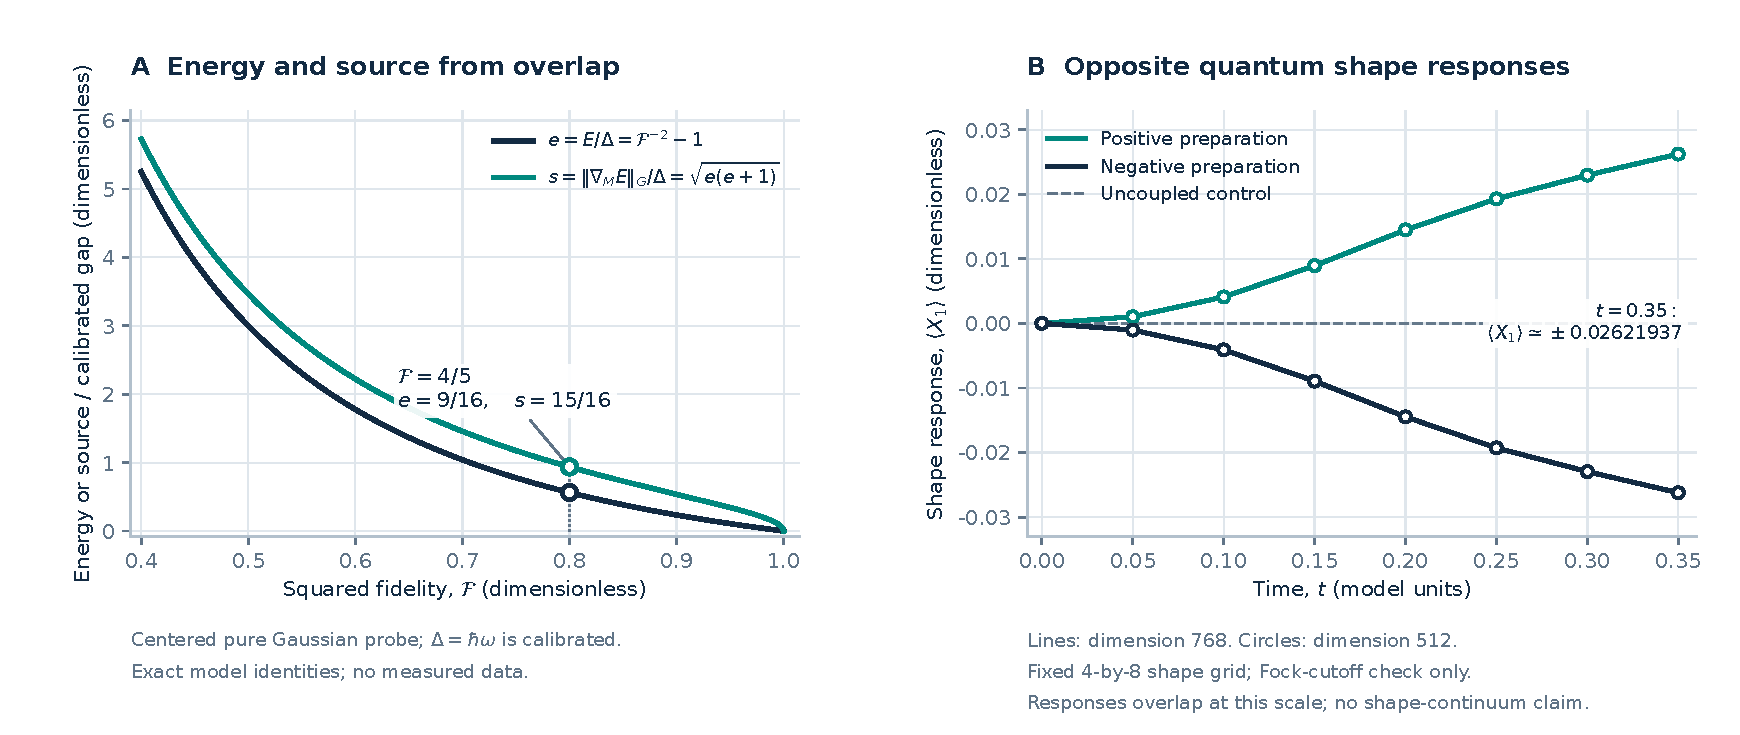
\includegraphics[width=\textwidth]{../figures/extensions.pdf}
\caption{Frozen analytical and numerical results. Left: dimensionless excitation energy and source magnitude versus squared fidelity. Right: recorded opposite shape responses and uncoupled control in the two finite quantum regulators. Overlapping cutoffs indicate the stated finite comparison, not a continuum theorem.}
\end{figure}

\section{What quantized motion does to the matched ground band}
The Gaussian ground ray is
\[
\psi_{u,v}(x)=\left(\frac v\pi\right)^{1/4}e^{(iu-v)x^2/2}.
\]
Let $P$ be the fiberwise projection onto this ray and $Q=1-P$. The isometry $\xi\mapsto\xi(u,v)\psi_{u,v}(x)$ identifies the ground band with $L^2(\mathbb H^2)$. Set $c_I=\hbar^2/(2I)$.

\begin{proposition}[Exact compression and initial excitation]\label{prop:leak}
For smooth compactly supported $\xi$,
\begin{align}
PHP\,\xi&=c_I\left[-v^2(\xi_{uu}+\xi_{vv})-\frac{iv}{2}\xi_u+\frac5{16}\xi\right]\label{eq:compression}\\
&=c_I\left(-\Delta_{\mathcal A}+\tfrac14\right)\xi,
\qquad \mathcal A=-\frac{\dd u}{4v}.
\end{align}
For a normalized initial ground-band state with total energy $E_{\mathrm{joint}}=\langle H\rangle$,
\begin{equation}\label{eq:leak}
\boxed{\Pr(Q\text{ at }t)=\frac{E_{\mathrm{joint}}}{4I}t^2+o(t^2).}
\end{equation}
No nonzero compactly supported $\xi$ makes the first off-band derivative vanish.
\end{proposition}
\begin{proof}
Use $\Delta_G=v^2(\partial_u^2+\partial_v^2)$ and Gaussian moments $\langle x^2\rangle=1/(2v)$, $\langle x^4\rangle=3/(4v^2)$. Direct differentiation gives \eqref{eq:compression}. The scalar correction is $c_I G^{ij}(g_{\mathrm{FS}})_{ij}=c_I/4=\hbar^2/(8I)$, since $G=8g_{\mathrm{FS}}$ in two target dimensions.

Define $D=v(\partial_v-i\partial_u)+1/4$. The exact orthogonal component is
\[
QH(\xi\psi)=c_I vD\xi\left(x^2-\frac1{2v}\right)\psi.
\]
With measure $\dd u\dd v/v^2$, integration by parts gives
\[
D^\dagger=-v\partial_v-iv\partial_u+5/4,
\qquad D^\dagger D=c_I^{-1}PHP.
\]
The centered $x^2$ variance is $1/(2v^2)$, hence
\[
\|QH(\xi\psi)\|^2=\frac{c_I^2}{2}\|D\xi\|^2
=\frac{c_I}{2}E_{\mathrm{joint}}.
\]
The strong unitary expansion on $D(H)$ proves \eqref{eq:leak}. Finally, $D\xi=0$ makes $v^{1/4}\xi$ holomorphic. A compactly supported holomorphic function is zero.
\end{proof}

The projected operator is an exact compression, not exact autonomous evolution of an invariant band. The $t\to0$ coefficient is independent of $\omega$; this is not a uniform-in-time adiabatic statement. Berry and Born--Huang structures have established precedents~\cite{Garcia,Wiggins}; the exact coefficient and leakage identity here use this particular Gaussian target.

As an independent integral control, the normalized packet
\[
\xi(u,v)=2\pi^{-1/4}v^2e^{-v-u^2/2}
\]
has $E_{\mathrm{joint}}=45c_I/16$ and $\|QH\xi\psi\|^2=45c_I^2/32$. Its decay justifies the same integrations by parts. Its initial excitation coefficient is $45\hbar^2/(128I^2)$. The total joint energy in this proposition is distinct from the probe mismatch energy in \eqref{eq:energy}.

\section{A genuine one-Killing action selector}
Work locally with a spacelike Killing field and the dictionary
\begin{equation}\label{eq:KK}
g_4=\lambda^{-1}h_{ab}\dd x^a\dd x^b
+\lambda(\dd y+A_a\dd x^a)^2,\qquad a,b=0,1,2,\quad\lambda>0.
\end{equation}
The Einstein-frame quotient $h$ has signature $(-,+,+)$. On the regular helical patch $r>0$, use orientation $\epsilon_{Tr\theta}=+\sqrt{-h}$. For $F=\dd A$, the vacuum duality is $\dd\chi=\lambda^2 *_hF$. Its target metric is $G=\lambda^{-2}(\dd\lambda^2+\dd\chi^2)$.

Locality, base diffeomorphism invariance, full target $SL(2,\R)$ invariance, the stated fields, and polynomial dependence on derivatives of total order at most two restrict the scalar formulation, modulo divergences, to
\begin{equation}\label{eq:S3}
S_3=\int\sqrt{-h}\left[fR[h]-\frac w{2\lambda^2}\big((\nabla\lambda)^2+(\nabla\chi)^2\big)+V\right]\dd^3x,
\end{equation}
where $f,w,V$ are constants. Transitivity fixes target scalar coefficients; isotropy fixes the target bilinear form and excludes invariant one-forms. There is no parity-odd two-derivative scalar in this three-dimensional field class. The one-Killing reduction itself is established~\cite{Moncrief,GerochGroup}; the following is an inverse calibration theorem for \eqref{eq:S3}.

\begin{theorem}[Helical flat-calibration selection]\label{thm:helical}
For nonzero pitch $\Omega$, the fields
\begin{equation}\label{eq:helical}
\lambda=1+\Omega^2r^2,\qquad \chi=2\Omega T,\qquad
h=-\lambda\dd T^2+\lambda\dd r^2+r^2\dd\theta^2
\end{equation}
are stationary for all compactly supported independent variations of \eqref{eq:S3} if and only if $w=f$ and $V=0$. Positive nondegenerate target energy selects $f=w>0$.
\end{theorem}
\begin{proof}
Start with Minkowski space in cylindrical coordinates and set $z=y$, $\phi=\theta+\Omega y$. The adapted Killing field is $\partial_z+\Omega\partial_\phi$, with norm $\lambda$. The connection is $A=(\Omega r^2/\lambda)\dd\theta$. The displayed orientation gives $\dd\chi=\lambda^2*F$. Direct calculation yields
\[
\operatorname{Ric}_{ab}[h]=\frac{\lambda_a\lambda_b+\chi_a\chi_b}{2\lambda^2},
\]
and both hyperbolic wave-map equations vanish. The metric residuals of \eqref{eq:S3} include
\begin{equation}\label{eq:helres}
E_{TT}=\frac{\Omega^2(f-w)}\lambda+\frac{V\lambda}{2},\qquad
E_{rr}=\frac{\Omega^2(f-w)}\lambda-\frac{V\lambda}{2}.
\end{equation}
Their sum and difference force $w=f$ and $V=0$. Conversely, the Ricci and target identities make every field equation vanish with those constants. Positivity fixes the nondegenerate sign.
\end{proof}

The zero-pitch calibration leaves $f-w$ undetermined; the pitch assumption is essential. At nonzero pitch, bounded residuals $|E_{TT}|,|E_{rr}|\le\epsilon$ give
\[
|f-w|\le\lambda\epsilon/\Omega^2,\qquad |V|\le2\epsilon/\lambda.
\]
The calibration has extra symmetries, but \eqref{eq:S3} is a theory for arbitrary $(2+1)$-dimensional quotient fields. A second Killing restriction is not imposed on its action or variations.

\subsection{Off-shell reduction and the old sector}
An independent arbitrary-jet calculation confirms
\begin{equation}\label{eq:KKdensity}
\begin{split}
\sqrt{-g_4}R[g_4]={}&\sqrt{-h}\left[R[h]-\frac{(\nabla\lambda)^2}{2\lambda^2}
-\frac{\lambda^2}{4}F_{ab}F^{ab}\right]\\
&+\partial_a\left(\sqrt{-h}\nabla^a\log\lambda\right).
\end{split}
\end{equation}
The calculation retains arbitrary first/second norm and connection jets and second quotient-metric jets in normal coordinates and local connection gauge. Vacuum dualization yields the selected scalar action.

For the foundation's cylindrical sector,
\[
g_4=e^{\gamma-\psi}(-\dd T^2+\dd R^2)+e^\psi(\dd z+A\dd\phi)^2
+R^2e^{-\psi}\dd\phi^2,
\]
reducing only along $z$ gives
\[
\lambda=e^\psi,\quad h_3=e^\gamma(-\dd T^2+\dd R^2)+R^2\dd\phi^2,
\quad \chi=\text{the original dual twist field}.
\]
The resulting target is $\dd\psi^2+e^{-2\psi}\dd\chi^2$. Its wave equations and quotient Einstein equations recover exactly the original nonlinear two-field PDE and the $\gamma$ energy/flux constraints when fields are $\phi$-independent. The new covariance dictionary uses $(u,v)=(\chi,\lambda)$; it is not silently identified with the earlier two-orbit shape matrix.

\section{Reciprocal sources and the required twist correction}
Adding a probe expectation $E(M,N)$ generically sources $\chi$. The vacuum reconstruction $F=-\lambda^{-2}*\dd\chi$ is then not closed. This is an actual obstruction to combining the constructions without modification.

\subsection{A specified covariant smooth-current model}
An explicit enlarged matter architecture uses a timelike vector density $j^a$, with
\[
n=\frac{\sqrt{-h_{ab}j^aj^b}}{\sqrt{-h}},\qquad
u^a=\frac{j^a}{\sqrt{-h}n},\qquad u^au_a=-1.
\]
For a normalized state field $\Psi$ in the calibrated probe Hilbert space, let $e=m_0+\langle H_M^{\mathrm{ex}}\rangle$, $m_0>0$, and take
\begin{equation}\label{eq:fluid}
S_m=\int\left[j^a\big(\partial_a\theta+i\hbar\langle\Psi|\partial_a\Psi\rangle
+\beta_A\partial_a\alpha^A\big)-\sqrt{-h}\,ne\right]\dd^3x.
\end{equation}
Normalization is imposed by a multiplier. The Berry term can equivalently be written in symmetrized real form. Clebsch variables allow general local flow; omitting them gives a restricted velocity-potential subclass. Current-action methods have established precedent~\cite{Brown}.

The common action $S_3+S_m$, with $w=f>0$, gives
\begin{align}
\nabla_a(nu^a)&=0,& i\hbar u^a\partial_a\Psi&=H_M^{\mathrm{ex}}\Psi
\quad\text{up to phase},\\
T^{m}_{ab}&=ne\,u_au_b,&f\tau^A(q)&=nG^{AB}\langle\partial_BH_M^{\mathrm{ex}}\rangle,\label{eq:sourcestress}\\
2f\,\operatorname{Ein}_{ab}[h]&=fT^{\mathrm{shape}}_{ab}+T^m_{ab}.&&
\end{align}
Here $q=(\lambda,\chi)$, $\tau$ is the hyperbolic wave-map tension, and
\[
T^{\mathrm{shape}}_{ab}=G_{AB}\partial_aq^A\partial_bq^B-\tfrac12h_{ab}\mathcal X,
\qquad\mathcal X=G_{AB}h^{cd}\partial_cq^A\partial_dq^B.
\]
The state/current equations imply
\begin{equation}\label{eq:ward}
\nabla_aT^{ma}{}_b=-n\langle\partial_AH_M^{\mathrm{ex}}\rangle\partial_bq^A.
\end{equation}
The weighted shape stress $fT^{\mathrm{shape}}_{ab}$ has the opposite divergence by its sourced equation, so the Einstein Bianchi identity is consistent. This supplies reciprocal sources from one action. It is a local deterministic state-fluid variational model; global smoothness, caustics, and a general hybrid measurement theory are not proved. It is not derived as a continuum limit of the quantum cell.

\subsection{Master action and fixed contact term}
The shear $U_\chi=\exp(i\chi\widehat Q^2/2)$ gives $H_M=U_\chi H_0(\lambda)U_\chi^\dagger$. Set $\Psi=U_\chi\widetilde\Psi$. The Berry term becomes
\[
i\hbar\langle\Psi|\partial_a\Psi\rangle
=i\hbar\langle\widetilde\Psi|\partial_a\widetilde\Psi\rangle
-\hbar\langle\widehat Q^2/2\rangle\partial_a\chi.
\]
Define the smooth current $J^a=\hbar nu^a\langle\widehat Q^2/2\rangle$. The twist density is
\[
\mathcal L_\chi=-\frac f{2\lambda^2}(\dd\chi)^2-J\cdot\dd\chi,
\]
whose equation conserves $C=f\lambda^{-2}\dd\chi+J$. With $*^2=-1$ on one- and two-forms in the Lorentzian three-dimensional convention,
\begin{equation}\label{eq:currentmap}
\boxed{F=-*C/f,\qquad\dd F=0,\qquad
\dd\chi=\lambda^2(*F-J/f).}
\end{equation}
Thus a local $A$ exists on a contractible patch. The master density with independent one-form $v$ is
\[
\mathcal L_{\mathrm{master}}=-\frac f{2\lambda^2}v^2-J\cdot v+fv\cdot*F,
\qquad F=\dd A.
\]
Varying $A$ gives $\dd v=0$; varying $v$ gives $v=\lambda^2(*F-J/f)$. Eliminating $v$ yields
\begin{equation}\label{eq:dual}
\boxed{\mathcal L_{\mathrm{dual}}=-\frac{f\lambda^2}{4}F^2
-\lambda^2J\cdot*F+\frac{\lambda^2}{2f}J^2
=-\frac{f\lambda^2}{4}(F+*J/f)^2.}
\end{equation}
Both the mixed term and contact term are compulsory. Metric dependence of $J$ must be retained in the full variation. Point-current delta distributions would make $J^2$ undefined, so the stated smooth-current or finite-regulator premise cannot be dropped.

\subsection{The clock and uplift boundary}
The state-fluid clock is proper time of $h_3$. For a horizontal four-dimensional trajectory, \eqref{eq:KK} gives $\dd\tau_4=\lambda^{-1/2}\dd s_3$. A fixed four-dimensional proper-time gap would therefore be $\lambda^{-1/2}$-dependent in the three-dimensional clock. The constant target-equivariant gap is an explicit three-dimensional calibration. The repaired connection reconstructs a metric locally, but an ordinary minimally coupled four-dimensional matter uplift is not established. These distinctions prevent a three-dimensional variational extension from being relabeled a completed quantum-gravity continuum.

\section{A full four-dimensional quadratic-curvature selector}
Use signature $(-,+,+,+)$ and the normalized action
\begin{equation}\label{eq:quadratic}
S=\frac1{2\kappa}\int\sqrt{-g}\left[R+\alpha R^2+\beta R_{ab}R^{ab}
+\gamma E_4\right]\dd^4x+S_m[g,\mathrm{matter}].
\end{equation}
Coefficients are constant, $\kappa>0$, and $\alpha,\beta$ have length-squared units. This is the parity-even quadratic-curvature class modulo the Euler density and boundary $\Box R$ term. The physical metric, source actions, and normalization are fixed; variations are unrestricted four-dimensional ones.

The equations are $\operatorname{Ein}_{ab}+\alpha H^{(1)}_{ab}+\beta H^{(2)}_{ab}=\kappa T_{ab}$, with
\begin{align}
H^{(1)}_{ab}&=2RR_{ab}-\tfrac12g_{ab}R^2+2(g_{ab}\Box-\nabla_a\nabla_b)R,\\
H^{(2)}_{ab}&=\Box R_{ab}+\tfrac12g_{ab}\Box R-\nabla_a\nabla_bR
+2R_{acbd}R^{cd}-\tfrac12g_{ab}R_{cd}R^{cd}.
\end{align}
Their trace is
\begin{equation}\label{eq:trace}
-R+(6\alpha+2\beta)\Box R=\kappa T.
\end{equation}
These field equations and the Ricci-flat degeneracy are established quadratic-gravity results~\cite{Pravda,Salvio}. The informative new-to-bundle calibration uses matter response.

\begin{theorem}[Two-source calibration selector]\label{thm:quadratic}
Within \eqref{eq:quadratic}, retaining both the specified dust-FLRW solution and charged electrovac solution with their same calibrated minimal sources is equivalent to $\alpha=\beta=0$. The constant Euler coefficient remains bulk-invisible.
\end{theorem}
\begin{proof}
For dust on $t>0$,
\[
\dd s^2=-\dd t^2+t^{4/3}(\dd x^2+\dd y^2+\dd z^2),\qquad
\kappa\rho_d=4/(3t^2),\quad p_d=0,
\]
direct curvature gives $R=4/(3t^2)$ and $\Box R=-8/(3t^4)$. The fixed Einstein dust source already satisfies $-R=\kappa T$, so \eqref{eq:trace} forces $3\alpha+\beta=0$.

For charged electrovac, choose geometric units $M=1$, $Q=1/2$ and
\[
f_r=1-\frac2r+\frac1{4r^2},\qquad
\dd s^2=-f_r\dd t^2+f_r^{-1}\dd r^2+r^2\dd\Omega_2^2,
\qquad F_{tr}=\frac1{2r^2}.
\]
With minimal Maxwell action $-F^2/4$ and $\kappa=2$ in these units, all Einstein--Maxwell equations hold; for general fixed $\kappa$, rescale the physical charge while retaining the geometric $Q$. Here $R=0$, so $H^{(1)}=0$, whereas
\begin{equation}\label{eq:RN}
H^{(2)a}{}_b=\frac{4r^2-8r+1}{4r^8}\operatorname{diag}(-3,-1,2,2).
\end{equation}
At $r=3$, $f_r=13/36>0$ and $H^{(2)t}{}_t=-13/8748\ne0$. The same fixed Maxwell source therefore forces $\beta=0$, and the dust condition gives $\alpha=0$. The converse follows by restoring the Einstein equations; no singular center is used.
\end{proof}

The decisive electrovac component was independently recovered by varying the raw radial Ricci-squared action with lapse and radial metric independent before substitution. A separately implemented review varied the metric arrays directly and obtained the same result. These are distinct checks of \eqref{eq:RN}.

Let $y_D$ be the trace residual at dust $t=1$ and $y_R$ the mixed $t$--$t$ residual at electrovac $r=3$. In the stated dimensionless calibration units,
\begin{equation}\label{eq:inversequad}
\begin{pmatrix}y_D\\y_R\end{pmatrix}
=\begin{pmatrix}-16&-16/3\\0&-13/8748\end{pmatrix}
\begin{pmatrix}\alpha\\\beta\end{pmatrix},
\quad
\beta=-\frac{8748}{13}y_R,\quad
\alpha=-\frac{y_D}{16}+\frac{2916}{13}y_R.
\end{equation}
The determinant is $52/2187$. Thus $|y_D|\le\epsilon_D$, $|y_R|\le\epsilon_R$ imply individually sharp bounds
\[
|\beta|\le\frac{8748}{13}\epsilon_R,\qquad
|\alpha|\le\frac{\epsilon_D}{16}+\frac{2916}{13}\epsilon_R.
\]
Sharpness follows by mapping the appropriate residual-rectangle corners through the invertible linear map. Restoring a reference length $L_0$ replaces coefficients by $\alpha/L_0^2,\beta/L_0^2$ and residuals by $L_0^2y$.

These sourced calibrations are additional premises, not deductions from the earlier flat vacuum. The theorem does not experimentally exclude higher-curvature corrections or set every effective-field-theory coefficient to zero.

\section{Distinguishing responses and concrete inverse problems}
About Minkowski spacetime, differentiating the quadratic action in all ten symmetric perturbation amplitudes gives
\begin{equation}\label{eq:linear}
(1+\beta\Box)G^L_{ab}+(2\alpha+\beta)(\eta_{ab}\Box-\partial_a\partial_b)R^L
=\kappa T_{ab}.
\end{equation}
For a conserved source with a fixed Green-function prescription and nonzero spacelike Fourier value $z=k^2>0$, decompose the response into transverse traceless and scalar sectors. Their Einstein-normalized curvature transfers are
\begin{equation}\label{eq:transfer}
\boxed{r_2(z)=\frac1{1-\beta z},\qquad
r_0(z)=\frac1{1+(6\alpha+2\beta)z}.}
\end{equation}
Added homogeneous waves are excluded by the response prescription. The curvature observables are gauge-invariant at linear order about flat space.

\begin{proposition}[Response inverse]
For finite nonzero responses and regular denominators, define
\[
y_2=(r_2^{-1}-1)/z,\qquad y_0=(r_0^{-1}-1)/z.
\]
Then
\begin{equation}
\boxed{\beta=-y_2,\qquad \alpha=(y_0+2y_2)/6.}
\end{equation}
Consequently, Einstein responses in both channels at this scale select zero non-topological quadratic coefficients in the stated class. Errors obey $|\delta\beta|\le\epsilon_2$ and $|\delta\alpha|\le(\epsilon_0+2\epsilon_2)/6$ for the corresponding inverse-response envelopes.
\end{proposition}
The proof is the direct affine inverse. This tests sourced response rather than only survival of a vacuum solution or on-shell Einstein perturbations.

\subsection{Estimating normalization as well}
If $\kappa$ is unknown, define $X_2=1/(G^L_{TT}/T_{TT})$ and $X_0=1/(-R^L/T)$. Then
\[
X_2(z)=(1-\beta z)/\kappa,\qquad
X_0(z)=[1+(6\alpha+2\beta)z]/\kappa.
\]
Two tensor measurements at distinct nonzero $z_1,z_2$ and one scalar measurement at $z_1$ identify
\begin{align}
q&=\frac{z_2X_2(z_1)-z_1X_2(z_2)}{z_2-z_1},&
s_2&=\frac{X_2(z_2)-X_2(z_1)}{z_2-z_1},\\
s_0&=\frac{X_0(z_1)-q}{z_1},&
\kappa&=q^{-1},\quad\beta=-s_2/q,\quad\alpha=(s_0+2s_2)/(6q).
\end{align}
The design determinant is $z_1(z_2-z_1)$. A fourth observation supplies the consistency test
\[
z_2X_0(z_1)-z_1X_0(z_2)-z_2X_2(z_1)+z_1X_2(z_2)=0.
\]
It tests this response class rather than assuming it from a single fit.

\subsection{Exterior-potential application and exclusions}
In the non-tachyonic range $\beta<0$, $c=6\alpha+2\beta>0$, define $m_2^2=-1/\beta$, $m_0^2=1/c$. Use the Newtonian/isotropic convention $\dd s^2=-(1+2\Phi)\dd t^2+(1-2\Psi)\dd\mathbf x^2$. For a calibrated static point source with decaying asymptotically flat linear response, the established quadratic-gravity potentials~\cite{Salvio} are
\begin{align}
\Phi&=-\frac{GM}{r}\left[1+\tfrac13e^{-m_0r}-\tfrac43e^{-m_2r}\right],\\
\Psi&=-\frac{GM}{r}\left[1-\tfrac13e^{-m_0r}-\tfrac23e^{-m_2r}\right].
\end{align}
With $U=-r\Phi/(GM)$, $V=-r\Psi/(GM)$,
\[
e^{-m_0r}=U-2V+1,\qquad e^{-m_2r}=(2-U-V)/2.
\]
When both lie strictly between zero and one, their logarithms determine both masses and coefficients. Obtaining both potentials is a separate calibrated observational task; one force measurement is not automatically two potential measurements.

An exact negative control shows why the operator class matters. Adding a higher-derivative contribution can change an inverse response to
\[
1+(c-dz_0)z+dz^2,
\]
which matches $1+cz$ at $z=z_0$ for every $d$ but differs elsewhere. Fixed-source and fixed-metric conditions also matter: a perturbative metric field redefinition shifts curvature-squared terms into matter-curvature couplings. Finally, demanding no extra poles would select $\alpha=\beta=0$ only in the exact finite polynomial class. Poles beyond an EFT cutoff cannot justify vanishing Wilson coefficients~\cite{Donoghue}.

\section{Verification, provenance, and remaining work}
The extension's reproducibility runner executes frozen sources in isolated temporary directories. Exact arithmetic, bounded floating-point calculations, analytic operator arguments, and Lean certificates are distinguished in the claim ledger.
\begin{center}\small
\begin{tabular}{@{}>{\raggedright\arraybackslash}p{0.54\textwidth}>{\raggedright\arraybackslash}p{0.39\textwidth}@{}}
\toprule
Evidence & Executed result\\\midrule
Selected dynamics checker & 41 exact checks plus two finite quantum regulators\\
Quadratic response / sourced calibrations & 88 / 73 exact checks\\
One-Killing / generic reduction and duality & 309 / 15 exact checks\\
Projected kinetic and leakage control & 13 exact checks\\
Separate bounded review & 31 independently implemented exact checks\\
Independent radial-action variation & Nonzero electrovac component reproduced\\
Formal project & 63 theorems in nine modules, zero warnings/errors\\\bottomrule
\end{tabular}
\end{center}
Counts include tensor components and overlapping controls, not distinct discoveries. The 15 new Lean theorems certify explicit helical and sourced residual inverses, selectors and bounds, regular response inversion, mismatch-energy positivity, and covariance energy/source identities. The full tensor variations, operator theory, current-fluid Ward identity, and physical interpretation are not all formalized.

Lean 4.19.0 and the exact pinned mathlib revision are retained. All 63 axiom reports contain only \texttt{propext}, \texttt{Classical.choice}, and \texttt{Quot.sound}. The true-proposition control passes and the deliberate false control is rejected. The previous 48 theorem sources remain unchanged.

The supplied review motivated the three questions and provided the flat Hessian-sector control; that contribution is credited separately from the nonlinear source-calibration and reciprocal-dynamics derivations. A separately tasked AI reviewer independently checked integration points and identified the bounded-observable domain correction. This is not external human peer review. All calculations, corrections, and review were frozen before public authoring.

The framework now has a selected reciprocal interaction, a source-sensitive quadratic discriminator, and a one-Killing inverse calibration. Their boundaries remain substantive: an interacting constrained quantum continuum, a limiting theorem connecting the quantum cell to the state-fluid architecture, an ordinary minimally coupled four-dimensional matter uplift, and empirical tests are open. Existing Gaussian, Born--Huang, Geroch-reduction, and quadratic-gravity physics are credited. The contribution is the explicit conditional selection and observable chain in this framework, not an assertion that those established mechanisms were first discovered here.

\section*{Reproduction and availability}
From the repository root, install the pinned Python requirements and run
\begin{quote}\small\ttfamily
python scripts/reproduce.py --output-dir work/reproduction
\end{quote}
For only the new extension suite use \texttt{scripts/verify\_extensions.py}. After preparing the pinned Lean dependencies, run
\begin{quote}\small\ttfamily
python scripts/verify\_lean.py --project formal --output work/lean
\end{quote}
The repository contains both papers, detailed derivations, raw states, all scripts and receipts, formal coverage, phase-freeze records, and SHA-256 manifests. Version 1.0 remains preserved as a separate release. Research by Logan Voss, with AI-assisted mathematical development, verification, formalization, and editing.

\begin{thebibliography}{12}
\bibitem{Voss1} L. Voss, \emph{On Quantum Mechanics and General Relativity}, research edition 1.0 (2026). \href{https://github.com/LoganVoss/on-quantum-mechanics-and-general-relativity/releases/tag/v1.0.0}{Preserved research release}.
\bibitem{HacklBianchi} L. Hackl, E. Bianchi, \emph{Bosonic and fermionic Gaussian states from K\"ahler structures}, SciPost Phys. Core 4, 025 (2021). \href{https://arxiv.org/abs/2010.15518v4}{arXiv:2010.15518v4}.
\bibitem{HacklDynamics} L. Hackl et al., \emph{Geometry of variational methods: dynamics of closed quantum systems}, SciPost Phys. 9, 048 (2020). \href{https://arxiv.org/abs/2004.01015v4}{arXiv:2004.01015v4}.
\bibitem{Banchi} L. Banchi, S. L. Braunstein, S. Pirandola, \emph{Quantum fidelity for arbitrary Gaussian states}, Phys. Rev. Lett. 115, 260501 (2015). \href{https://arxiv.org/abs/1507.01941v1}{arXiv:1507.01941v1}.
\bibitem{Garcia} A. Garcia-Chung, \emph{On the geometric phase for Gaussian states} (2020). \href{https://arxiv.org/abs/2004.14204v1}{arXiv:2004.14204v1}.
\bibitem{Wiggins} S. Wiggins, \emph{What solvable models reveal about Born--Oppenheimer, Born--Huang, and exact factorization} (2026). \href{https://arxiv.org/abs/2608.08668v2}{arXiv:2608.08668v2}.
\bibitem{Moncrief} V. Moncrief, \emph{The Reduction Problem for Einstein's Equations}, pp. 168--174. \href{https://maths.anu.edu.au/files/CMAProcVol19-Moncrief.pdf}{Author's proceedings article}.
\bibitem{GerochGroup} R. G. Leigh, A. C. Petkou, P. M. Petropoulos, P. K. Tripathy, \emph{The Geroch group in Einstein spaces} (2014). \href{https://arxiv.org/abs/1403.6511v2}{arXiv:1403.6511v2}.
\bibitem{Brown} J. D. Brown, \emph{Action functionals for relativistic perfect fluids}, Class. Quant. Grav. 10, 1579--1606 (1993). \href{https://arxiv.org/abs/gr-qc/9304026v1}{arXiv:gr-qc/9304026v1}.
\bibitem{Pravda} V. Pravda et al., \emph{Exact solutions to quadratic gravity}, Phys. Rev. D 95, 084025 (2017). \href{https://arxiv.org/abs/1606.02646v3}{arXiv:1606.02646v3}.
\bibitem{Salvio} A. Salvio, \emph{Quadratic Gravity}, Front. Phys. 6, 77 (2018). \href{https://arxiv.org/abs/1804.09944v2}{arXiv:1804.09944v2}.
\bibitem{Donoghue} J. F. Donoghue, \emph{General relativity as an effective field theory: The leading quantum corrections}, Phys. Rev. D 50, 3874 (1994). \href{https://arxiv.org/abs/gr-qc/9405057}{arXiv:gr-qc/9405057}.
\end{thebibliography}
\end{document}
